% HOF-Net-R 논문 초안 (2026-11-27)
% 컴파일 : xelatex main → bibtex main → xelatex main → xelatex main   (TinyTeX, xetexko)
% 본문 수치의 출처 : numbers.md (extract_numbers.py 가 outputs/ 의 결과 파일에서 생성)
\documentclass[journal,a4paper,10pt]{IEEEtran}

\usepackage{amsmath,amssymb,mathtools,bm}
\usepackage{fontspec}
\usepackage[hangul]{xetexko}
\setmainfont{texgyretermes}[Extension=.otf, UprightFont=*-regular, BoldFont=*-bold, ItalicFont=*-italic, BoldItalicFont=*-bolditalic]
\setsansfont{texgyreheros}[Extension=.otf, UprightFont=*-regular, BoldFont=*-bold, ItalicFont=*-italic, BoldItalicFont=*-bolditalic]
\setmainhangulfont{HANBatang.ttf}[Path=C:/Windows/Fonts/, BoldFont=HANBatangB.ttf, ItalicFont=HANBatang.ttf, BoldItalicFont=HANBatangB.ttf]
\setsanshangulfont{malgun.ttf}[Path=C:/Windows/Fonts/, BoldFont=malgunbd.ttf]
\setmonohangulfont{malgun.ttf}[Path=C:/Windows/Fonts/]
\usepackage{graphicx}
\usepackage{booktabs,multirow,array,makecell}
\usepackage{tikz}
\usetikzlibrary{positioning,arrows.meta,fit,calc}
\usepackage{xcolor}
\usepackage{cite}
\usepackage{enumitem}
\usepackage{stfloats}
\usepackage[hidelinks]{hyperref}

% 한국어 레이블
\AtBeginDocument{%
  \renewcommand{\figurename}{그림}%
  \renewcommand{\tablename}{표}%
  \renewcommand{\refname}{참고문헌}%
  \renewcommand{\appendixname}{부록}%
}
\newcommand{\sig}{\operatorname{sig}}
\newcommand{\softplus}{\operatorname{softplus}}
\newcommand{\KL}{\operatorname{KL}}
\newcommand{\E}{\mathbb{E}}
\newcommand{\Var}{\operatorname{Var}}
\newcommand{\N}{\mathcal{N}}
\newcommand{\RZIB}{R-ZIB}
\newcommand{\ko}[1]{\textsf{#1}}
\setlength{\tabcolsep}{3.2pt}
\renewcommand{\arraystretch}{1.08}
\hyphenation{Light-GBM Stat-cast}

\markboth{HOF-Net-R : 약한 신호·영과잉 목표를 위한 단계적 확률 신경망 (초안, 2026-11-27)}%
{최용원 : HOF-Net-R, 단계적 확률 신경망과 투구 구위 평가}

\begin{document}

% ---------------------------------------------------------------------------
% 제목 영역 (1단) : 제목, 저자, 국문 초록, Abstract, 주제어
% ---------------------------------------------------------------------------
\twocolumn[{%
\begin{center}
{\fontsize{19pt}{24pt}\selectfont\sffamily\bfseries HOF-Net-R : 약한 신호·영과잉 목표를 위한\\[2pt] 단계적 확률 신경망과 투구 구위 평가\par}
\vspace{6pt}
{\large HOF-Net-R: A Staged Probabilistic Neural Network for Weak-Signal,\\ Zero-Inflated Tabular Targets, with Application to Pitch Stuff Evaluation\par}
\vspace{10pt}
{\large 최용원 \;(Yongwon Choi)\par}
\vspace{3pt}
{\small 연구 초안 · 2026년 11월 27일\par}
\end{center}
\vspace{6pt}
\noindent\rule{\textwidth}{0.4pt}\par\vspace{4pt}
\noindent\begin{minipage}{\textwidth}
\small
\noindent{\sffamily\bfseries 요\enspace 약}\quad
투구 물리량만으로 구위(stuff)를 평가하는 문제는 타구 결과의 우연 변동이 커서 설명력이 낮고(검증 $R^2\approx0.02$), 목표값의 절반 가량이 정확히 0(헛스윙)인 영과잉 분포를 가진다. 본 논문은 특성 토큰 어텐션 신경망 HOF-Net을 이 문제에 적용하며 관찰한 실패를 분석하고, 이를 단계적으로 개정한 HOF-Net-R을 제안한다. 투구마다 입력 조건부 잠재가중치의 변분 분포를 두는 원형 HOF-Net은 관측치마다 치르는 KL 비용(투구당 0.073 nat)이 신호로 얻을 수 있는 로그우도 이득(약 0.011 nat)보다 커서 상수 예측으로 붕괴했고, 강한 신호의 합성 데이터에서도 같은 붕괴를 보였다. HOF-Net-R은 (i) 결정적 어텐션 인코더로 평균을 먼저 학습하고, (ii) 데이터셋 전체가 공유하는 잔차 가중치에만 베이지안 추론을 적용하며(KL을 표본 수로 나눔), (iii) 영과잉 Beta(ZIB) 우도로 0과 양수 부분을 함께 모형화한다. 2024–2026 MLB Statcast 자료(2025 시즌 학습, 검증 35,291구)에서 ZIB 헤드를 쓴 HOF-Net-R은 LightGBM과 같은 수준의 점 예측(RMSE 0.1683 대 0.1682, 차이의 95\% 신뢰구간 $[-0.0001, 0.0002]$)과 약 16\% 낮은 CRPS(0.0733 대 0.0871)를 보였다. 그러나 대조 실험에서 LightGBM 평균에 ZIB 헤드를 붙여도 같은 CRPS(0.0732)를 얻어, 분포 예측의 개선은 구조가 아니라 우도의 효과임을 확인했다. 투수×구종 평균 구위와 헛스윙률의 순위 상관은 LightGBM보다 0.014 낮았으나 유의하지 않았고(95\% 신뢰구간 $[-0.038, 0.011]$), 시드 간 표준편차가 0.016으로 컸다. 공유 잔차 가중치의 불확실성은 예측 분산의 0.01\% 수준이어서 분포 밖 탐지에 쓸 수 없었다. 끝으로 8개 요인 그룹의 Shapley 설명과, 브라우저에서 같은 예측을 재현하는 추론 구현(예측값 오차 $<10^{-7}$)으로 웹 서비스에 적용한 결과를 보고한다.

\vspace{5pt}
\noindent{\sffamily\bfseries Abstract}\quad
Evaluating pitch quality (``stuff'') from pitch physics alone is a weak-signal problem (validation $R^2\approx0.02$) with a zero-inflated target, as roughly half of the training targets are exact zeros from swinging strikes. We analyze the failure of HOF-Net, a feature-token attention network with instance-conditional variational latent weights, and propose a staged revision, HOF-Net-R. The original model collapsed to a constant predictor because its per-observation KL cost (0.073 nat per pitch) exceeded the attainable log-likelihood gain (about 0.011 nat), and it collapsed even on strong-signal synthetic data. HOF-Net-R (i) learns the conditional mean with a deterministic attention encoder, (ii) restricts Bayesian inference to residual weights shared across the dataset with the KL scaled by the sample size, and (iii) adopts a zero-inflated Beta (ZIB) likelihood. On 2024–2026 MLB Statcast data, HOF-Net-R with the ZIB head matches LightGBM in point accuracy (RMSE 0.1683 vs.\ 0.1682) and lowers CRPS by about 16\%, but a control shows that LightGBM with the same ZIB head attains the same CRPS, so the gain comes from the likelihood rather than the architecture. Its rank correlation between pitcher-pitch-type stuff and whiff rate is 0.014 lower than LightGBM (not significant) with a larger seed variance, and its epistemic uncertainty is negligible. We also report group-Shapley explanations and a browser inference implementation reproducing the model to within $10^{-7}$.

\vspace{5pt}
\noindent{\sffamily\bfseries 주제어}\quad 정형 데이터 딥러닝, 변분 추론, 사후 붕괴, 영과잉 Beta 회귀, 적정 점수 규칙, Shapley 설명, 야구 분석, 구위\par
\noindent{\sffamily\bfseries Keywords}\quad tabular deep learning, variational inference, posterior collapse, zero-inflated beta regression, proper scoring rules, Shapley values, baseball analytics
\end{minipage}
\par\vspace{4pt}\noindent\rule{\textwidth}{0.4pt}\par\vspace{12pt}
}]

% ---------------------------------------------------------------------------
\section{서론}
\label{sec:intro}

투수가 던진 공의 질, 곧 구위(stuff)는 공의 속도·움직임·릴리스·회전 같은 물리량이 타자의 결과를 얼마나 억제하는지로 정의할 수 있다. 위치·볼카운트·상황을 제외하고 물리량만으로 구위를 점수화하는 접근은 공개 분석에서 널리 쓰인다~\cite{fangraphs2023stuff}. 이 문제는 두 가지 점에서 일반적인 회귀와 다르다. 첫째, 같은 물리량의 공도 타격 결과가 크게 달라 신호가 약하다. 본 연구의 목표값에서 가장 좋은 모형의 검증 결정계수는 $R^2\approx0.022$에 그친다. 둘째, 목표값은 헛스윙이면 정확히 0이고 인플레이 타구면 $(0,1)$의 연속값이어서, 검증 표본의 50.1\%가 0인 영과잉 분포를 이룬다.

정형 데이터에서는 그래디언트 부스팅이 여전히 강한 기준선이다~\cite{ke2017lightgbm,grinsztajn2022tree}. 신경망 쪽에서는 특성을 토큰으로 바꾸어 어텐션을 쓰는 구조가 제안되었다~\cite{gorishniy2021revisiting}. 본 연구의 출발점인 HOF-Net은 이 구조에 투구마다 입력 조건부 잠재가중치의 변분 분포와 어텐션에서 유도한 공분산을 더해, 특성 간 상호작용과 불확실성을 함께 설명하려는 모형이었다. 그러나 실제 자료에서 HOF-Net은 상수 예측으로 붕괴했다.

본 논문의 기여는 다음과 같다.
\begin{enumerate}[leftmargin=*,itemsep=1pt,topsep=2pt]
\item 원형 HOF-Net의 붕괴를 관측과 합성 실험으로 확인하고, 관측치별 KL 비용과 신호가 주는 로그우도 이득의 크기 비교로 원인을 설명한다(\ref{sec:hofnet}절).
\item 평균 학습, 공유 잔차 가중치의 베이지안 추론, 영과잉 Beta 우도의 세 단계로 나눈 개정 모형 HOF-Net-R을 제안한다(\ref{sec:method}절).
\item LightGBM과 점 예측·분포 예측·순위 지표·설명을 비교하고, 대조 실험으로 분포 예측 개선이 우도의 효과임을 분리한다. 개선되지 않은 부분(순위 지표, 시드 분산, 불확실성)도 그대로 보고한다(\ref{sec:results}절).
\item 단일 시드 모형으로 웹 서비스에 적용하고, 브라우저 추론의 수치 재현성을 검증한다(\ref{sec:deploy}절).
\end{enumerate}

% ---------------------------------------------------------------------------
\section{관련 연구}
\label{sec:related}

\textbf{정형 데이터 딥러닝.} FT-Transformer는 각 특성을 임베딩 토큰으로 바꾼 뒤 Transformer 블록을 적용한다~\cite{gorishniy2021revisiting,vaswani2017attention}. 대규모 비교 연구는 중간 규모 정형 데이터에서 트리 기반 모형이 여전히 우세하며, 특히 정보가 없는 특성과 불규칙한 목표 함수에 강하다고 보고한다~\cite{grinsztajn2022tree}. 본 연구의 기준선 LightGBM~\cite{ke2017lightgbm}도 같은 맥락에 있다.

\textbf{변분 추론과 사후 붕괴.} 잠재변수 모형의 변분 하한(ELBO) 학습~\cite{kingma2014vae}에서는 디코더가 잠재변수 없이도 우도를 잘 설명할 때 변분 분포가 사전분포로 수렴하는 사후 붕괴가 알려져 있다~\cite{bowman2016generating}. 신경망 가중치의 변분 추론~\cite{blundell2015weight}과 달리, 본 연구의 원형 모형은 관측치마다 다른 잠재가중치를 두었다는 점에서 VAE식 붕괴의 영향을 받는다.

\textbf{예측 불확실성.} 마지막 층에만 베이지안 선형회귀를 두는 방법은 닫힌형 사후분포로 인식론적 불확실성을 얻는다~\cite{snoek2015scalable,bishop2006pattern}. 딥 앙상블~\cite{lakshminarayanan2017simple}은 시드 다양성으로 불확실성을 근사한다. 우연·인식론 불확실성의 분해는 \cite{kendall2017uncertainties}에서, 이분산 가우시안 우도에서 평균과 분산이 학습 신호를 다투는 문제는 \cite{seitzer2022pitfalls}에서 다루었다.

\textbf{영과잉 비율 자료와 적정 점수.} Beta 회귀~\cite{ferrari2004beta}는 $(0,1)$ 값을, 영·일 과잉 Beta 회귀~\cite{ospina2012general}는 경계값의 점질량을 함께 모형화한다. 서로 다른 지배 측도를 갖는 분포(점질량과 밀도의 혼합 대 가우시안)는 로그우도를 직접 비교할 수 없으므로, CRPS 같은 적정 점수 규칙~\cite{gneiting2007strictly}으로 비교한다.

\textbf{설명.} Shapley 값~\cite{shapley1953value}은 협력 게임의 공정한 배분으로, SHAP~\cite{lundberg2017unified}과 트리 모형의 정확한 계산법 TreeSHAP~\cite{lundberg2020local}으로 널리 쓰인다. 결측 특성을 배경 분포에서 채우는 개입적(interventional) 정의는 \cite{janzing2020feature}에서 논의되었다.

% ---------------------------------------------------------------------------
\section{자료와 문제 정의}
\label{sec:data}

\subsection{자료와 분할}
MLB Statcast~\cite{savant}의 2024–2026 정규시즌 투구 기록(시즌당 708,479 / 708,593 / 713,177구)을 쓴다. 모형 학습은 2025 시즌만으로 하고, 2024·2026 시즌은 학습에 쓰지 않은 표본 밖 평가에 쓴다. 2025 정규시즌의 마지막 한 달(2025-08-29 – 09-28)을 검증 구간, 그 직전 14일(08-15 – 08-28)을 조기 종료와 초매개변수 선택용 홀드아웃, 그 이전을 학습 구간으로 둔다.

학습 표본은 인플레이 타구와 헛스윙이다(루킹 삼진, 파울, 볼은 제외). 표본 수는 학습 151,051구, 홀드아웃 15,845구, 검증 35,291구이다. 신경망은 학습 구간만, 기준선 LightGBM은 학습과 홀드아웃(166,896구)을 함께 써 학습했으므로 비교는 신경망에 약간 불리하다.

\subsection{목표값}
목표값 $y\in[0,1)$은 타구의 질을 나타내는 점수이며, 클수록 타자에게 유리하다(투수에게 나쁘다). 두 단계로 만든다. 1단계에서 랜덤 포레스트~\cite{breiman2001random}가 타구 방향·속도·발사각·공격각으로 타구 결과 $c\in\{0,1,2,3\}$(아웃, 1루타, 2·3루타, 홈런)의 확률 $p_c$를 추정하고(학습 행은 5겹 교차 적합), 기대값 $E=\sum_c c\,p_c\in[0,3]$을 얻는다. 2단계에서 $E$의 분포를 $[0,1)$로 옮긴다.
\begin{equation}
y = F^{-1}_{\mathrm{Beta}(a_0,b_0)}\!\big(F_{\mathrm{Gamma}(k,\theta)}(E)\big),
\label{eq:target}
\end{equation}
여기서 Gamma 분포는 최대우도로, Beta 분포의 $(a_0,b_0)$는 $E/3$의 평균·분산에 적률법으로 적합한다. 헛스윙은 $y=0$이다. 학습 표본에서 $y$의 최댓값은 0.818이어서 1의 점질량은 필요 없고, 검증 표본에서 $y\le0.005$의 비율은 50.1\%이다.

\subsection{입력 변수}
입력 $x\in\mathbb{R}^{13}\times\{\mathrm{L},\mathrm{R}\}$는 $p=14$개 변수이다. 구속, 수평·수직 무브먼트(inch), 릴리스 좌우·높이, 익스텐션, 팔 각도, 회전수, 회전축, 투수 주 패스트볼 대비 구속·수평·수직 무브먼트 차이, 높이 보정 진입각(HAVAA), 투구손이다. 좌투수는 좌우 성분의 부호를 바꾸고 회전축을 $360^\circ-$회전축으로 바꾸어 우투수 기준으로 맞춘다. 주 패스트볼은 투수별로 포심·싱커·커터 중 가장 많이 던진 구종이다.

공이 들어간 위치는 구위에 포함하지 않는다. 그러나 수직 진입각(VAA)은 공이 존의 어디로 들어가는지에 크게 의존하므로, 구종 $t$별 선형회귀의 잔차를 쓴다.
\begin{equation}
\mathrm{HAVAA} = \mathrm{VAA} - (\alpha_t + \delta_t\, z_{\mathrm{plate}}),
\label{eq:havaa}
\end{equation}
여기서 $z_{\mathrm{plate}}$는 홈플레이트 통과 높이이며, $(\alpha_t,\delta_t)$는 학습 구간에서 적합한다(500구 이상 구종은 구종별 회귀, 30–499구 구종은 공통 기울기와 구종별 절편, 그 밖은 공통 계수). 구종 코드 자체는 입력에 넣지 않는다. 구종 이름이 아니라 궤적으로 평가하기 위함이다.

\subsection{구위 점수}
모형의 예측 $\hat y(x)$는 낮을수록 좋은 공이다. 이를 20–80 척도로 옮긴다.
\begin{equation}
s(x)=\min\!\Big\{80,\max\!\big\{20,\;50+10\,\Phi^{-1}\!\big(\hat F_n(-\hat y(x))\big)\big\}\Big\},
\label{eq:scale}
\end{equation}
여기서 $\hat F_n$은 2025 학습 구간 정규시즌 투구($n=521{,}147$, 존에서 크게 벗어난 볼 제외)의 $-\hat y$에 대한 중간 순위 경험분포함수이고 $\Phi$는 표준정규 분포함수이다. 따라서 학습 구간의 중앙값이 50, 한 표준편차가 10점이다.

% ---------------------------------------------------------------------------
\section{원형 HOF-Net과 그 실패}
\label{sec:hofnet}

\subsection{구조}
원형 HOF-Net은 각 입력 $x_k$를 토큰 $e_k = x_k w_k + b_k\in\mathbb{R}^d$로 바꾸고 다중 헤드 셀프 어텐션으로 문맥 표현과 헤드 평균 어텐션 행렬 $\mathbf{A}(x)\in\mathbb{R}^{p\times p}$를 얻는다. 투구 $i$마다 잠재가중치 $W_i\in\mathbb{R}^p$를 두고 예측을 $m(x_i,W_i)=b+\sum_k W_{ik}\,h_k(x_{ik})$로 쓴다. 변분 분포는 $q_\phi(W_i\mid x_i)=\N(\mu_\phi(x_i),\,D_\phi R(x_i) D_\phi)$이며, 상관 행렬 $R$은 대칭화한 어텐션의 그람 행렬을 정규화해 만든다. 사전분포 $p_\psi(W_i\mid x_i)=\N(0,\mathrm{diag}\,\tau^2(x_i))$의 척도는 어텐션 중요도로 정한다. 학습은 관측치별 하한을 평균한 목적함수
\begin{multline}
\mathcal{J}_{\text{원형}}=\frac{1}{N}\sum_{i=1}^{N}\Big(-\E_{q_\phi}\log p(y_i\mid x_i,W_i)\\
+\gamma\,\KL\big(q_\phi(W_i\mid x_i)\,\|\,p_\psi(W_i\mid x_i)\big)\Big)
\label{eq:orig}
\end{multline}
을 $(\theta,\phi)$와 $\psi$에 대해 번갈아 최소화한다($\gamma=1$이 ELBO).

\subsection{관측된 붕괴}
표~\ref{tab:collapse}는 같은 입력 14개로 학습한 원형 모형의 변형들이다. $\gamma=1$인 원형(A0)은 홀드아웃 RMSE가 상수 예측과 소수 다섯째 자리까지 같고 예측의 표준편차가 $9\times10^{-5}$로, 사실상 상수를 예측한다. 대각 공분산(A1)도 같다. $\gamma$를 0.01까지 낮추면 일부 신호를 학습하지만, 변분 분포를 버리고 $W=\mu_\phi(x)$로 결정적으로 학습한 경우(결정적 HOF-Net)가 가장 낫다. 검증 투수×구종 구위와 헛스윙률의 순위 상관은 원형이 $-0.122$로 방향마저 틀렸다.

\begin{table}[!t]
\centering
\caption{원형 HOF-Net 변형의 붕괴 점검 (입력 14개, 2025 홀드아웃). 상수 예측의 RMSE는 0.17048이다. KL은 마지막 epoch의 투구당 값(nat).}
\label{tab:collapse}
\footnotesize
\begin{tabular}{@{}lcccc@{}}
\toprule
변형 & $\gamma$ & KL/투구 & RMSE & 예측 표준편차 \\
\midrule
A0 (원형) & 1 & 0.0726 & 0.17047 & $9.1\times10^{-5}$ \\
A1 (대각 공분산) & 1 & 0.0049 & 0.17046 & $3.3\times10^{-4}$ \\
A0, $\gamma{=}0.1$ & 0.1 & 0.2042 & 0.17043 & $1.4\times10^{-3}$ \\
A0, $\gamma{=}0.01$ & 0.01 & 0.6772 & 0.16988 & $8.8\times10^{-3}$ \\
결정적 ($W{=}\mu_\phi$) & – & 0 & \textbf{0.16899} & $2.5\times10^{-2}$ \\
\bottomrule
\end{tabular}
\end{table}

\subsection{원인}
\textbf{신호의 크기와 KL 비용.} 가우시안 우도에서 잔차 분산을 최적으로 맞춘다고 하면, 목표 분산의 $R^2$만큼을 설명하는 평균 함수가 상수 예측보다 얻는 관측치당 로그우도 이득은
\begin{equation}
\Delta\ell=-\tfrac12\log(1-R^2)
\label{eq:gain}
\end{equation}
이다. 본 자료의 $R^2\approx0.022$이면 $\Delta\ell\approx0.011$ nat이다. 반면 식~\eqref{eq:orig}은 관측치마다 KL을 치르며, A0의 KL은 투구당 0.073 nat로 이득의 여섯 배 이상이다. 최적화는 $q_\phi=p_\psi$로 KL을 없애고 신호를 포기하는 쪽이 유리하다.

\textbf{목적함수의 구조.} 이 설명만으로는 부족하다. 그림~\ref{fig:collapse}(a)처럼 $R^2\approx0.98$인 강신호 합성 자료에서도 원형은 평균 $R^2=0.011$로 붕괴했지만, 같은 인코더를 결정적으로 학습하면 $R^2\ge0.968$을 얻었다. 원인은 구조에도 있다. 첫째, $q_\phi(W_i\mid x_i)$는 $y_i$를 보지 않으므로 $W_i$의 사후분포 근사가 아니라 $x_i$의 확률적 재매개화일 뿐이며, 그 무작위성은 예측 잡음만 더한다. 둘째, $\psi$ 단계는 $\sum_i\KL(q\,\|\,p_\psi)$를 줄이므로 사전분포가 변분 분포 쪽으로 끌려가 KL에 아무 제약도 걸지 못한다. 셋째, 양의 정부호 상관 구조가 곧 유익한 상관을 뜻하지는 않는다. 어텐션이 거의 균일하면 $R$은 모든 원소가 1에 가까운 행렬이 된다.

\begin{figure}[!t]
\centering
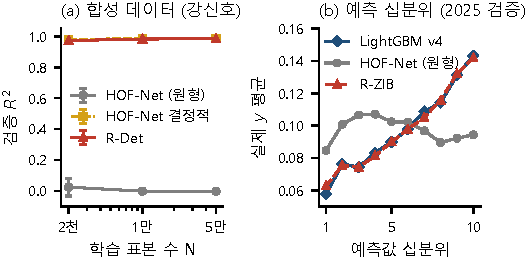
\includegraphics[width=\columnwidth]{figs/fig_collapse.pdf}
\caption{(a) 강신호 합성 자료에서의 검증 $R^2$ (5 시드 평균 ± 표준편차). (b) 2025 검증 구간에서 예측값 십분위별 실제 $y$의 평균 (시드 42). 원형은 십분위가 실제 값의 순서를 거의 반영하지 못한다.}
\label{fig:collapse}
\end{figure}

% ---------------------------------------------------------------------------
\section{HOF-Net-R}
\label{sec:method}

\subsection{설계 원칙}
위 분석에서 세 원칙을 얻는다. (1) 신호가 약할수록 평균 함수를 먼저, 확률적 요소 없이 학습한다. (2) 베이지안 추론은 관측치 전체가 정보를 나눠 갖는 전역 모수에만 적용해, KL 비용을 관측치 수로 나누어 치른다. (3) 우도는 목표값의 지지집합(0의 점질량과 $(0,1)$의 연속 부분)에 맞춘다. 그림~\ref{fig:arch}가 전체 구조이다.

\begin{figure*}[!t]
\centering
\resizebox{\textwidth}{!}{%
\begin{tikzpicture}[
  font=\footnotesize,
  box/.style={draw, rounded corners=2pt, align=center, minimum height=9.5mm, inner sep=3pt, fill=white},
  hl/.style={box, fill=gray!12},
  arr/.style={-{Stealth[length=2.2mm]}, thick},
  lab/.style={font=\scriptsize\itshape, text=gray!40!black},
  node distance=6mm and 6mm]
\node[box] (x) {입력 14개\\[-1pt]{\scriptsize 구속·무브먼트·릴리스}\\[-1pt]{\scriptsize 회전·차이·HAVAA·투구손}};
\node[box, right=of x] (tok) {토큰화\\[-1pt]{\scriptsize $e_k=\tilde x_k w_k+b_k+m_k u_k$}\\[-1pt]{\scriptsize $14\times32$}};
\node[box, right=of tok] (enc) {어텐션 블록 $\times2$\\[-1pt]{\scriptsize pre-LN, 4헤드}\\[-1pt]{\scriptsize FF $32\to64\to32$}};
\node[box, right=of enc] (h) {$h(x)\in\mathbb{R}^{448}$\\[-1pt]{\scriptsize 토큰 평탄화}};
\node[hl, above right=1mm and 7mm of h] (z) {잔차 기저\\[-1pt]{\scriptsize $z(x)\in\mathbb{R}^{16}$}};
\node[hl, below right=1mm and 7mm of h] (g) {ZIB 헤드 $g(h)$\\[-1pt]{\scriptsize $448\to64\to64\to3$}};
\node[box, right=7mm of z] (om) {공유 가중치 $\omega\in\mathbb{R}^{17}$\\[-1pt]{\scriptsize $q(\omega)=\N(m,\mathrm{diag}\,s^2)$}};
\node[box, right=7mm of g] (zib) {$\pi,\ \mu_+,\ \kappa$\\[-1pt]{\scriptsize $\mu_+=\sig(\ell_\mu+\tilde z^\top\omega)$}};
\node[box, right=6mm of zib] (ey) {$\E[Y\mid x]$\\[-1pt]{\scriptsize $=(1-\pi)\mu_+$}};
\node[box, above=7mm of ey] (s) {구위 20–80\\[-1pt]{\scriptsize 식~(\ref{eq:scale})}};
\draw[arr] (x) -- (tok); \draw[arr] (tok) -- (enc); \draw[arr] (enc) -- (h);
\draw[arr] (h.east) -- ++(3mm,0) |- (z.west);
\draw[arr] (h.east) -- ++(3mm,0) |- (g.west);
\draw[arr] (z) -- (om);
\draw[arr] (g) -- (zib);
\draw[arr] (om.south) -- (om.south |- zib.north);
\draw[arr] (zib) -- (ey); \draw[arr] (ey) -- (s);
\node[lab, below=1mm of enc] {Stage I : 평균(MSE)으로 학습 후 고정};
\node[lab, above=1mm of om] {Stage II : 전역 베이지안 잔차 (KL$/N$)};
\node[lab, below=1mm of zib] {Stage III : 영과잉 Beta 우도};
\end{tikzpicture}}
\caption{HOF-Net-R의 구조. 인코더(왼쪽)는 Stage I에서 평균 회귀로 학습한 뒤 고정한다. 본 모델 R-ZIB는 고정된 표현 $h(x)$ 위에 영과잉 Beta 헤드를 두고, 양수 부분 평균의 로짓에 데이터셋 전체가 공유하는 잔차 가중치 $\omega$를 더한다($\tilde z=[z,1]$). 운영 예측은 $\omega$의 사후평균을 쓰는 결정적 순전파 한 번이다.}
\label{fig:arch}
\end{figure*}

\subsection{인코더와 Stage I : 평균}
수치 입력은 학습 구간의 평균·표준편차로 표준화한 $\tilde x_k$로 바꾸고, 결측이면 $\tilde x_k=0$, $m_k=1$로 두어 학습되는 결측 임베딩 $u_k$를 더한다. 투구손은 임베딩으로 바꾼다(모르는 값은 별도 코드). 토큰 $Z\in\mathbb{R}^{p\times d}$($d=32$)에 pre-LN Transformer 블록~\cite{vaswani2017attention,xiong2020layer} 두 개를 적용한다.
\begin{equation}
Z\leftarrow Z+\mathrm{MHA}(\mathrm{LN}(Z)),\qquad Z\leftarrow Z+\mathrm{FF}(\mathrm{LN}(Z)),
\label{eq:block}
\end{equation}
여기서 MHA는 4헤드 셀프 어텐션, FF는 $d\to2d\to d$의 GELU~\cite{hendrycks2016gelu} 신경망이다. 평탄화한 표현 $h(x)=\mathrm{vec}(Z)\in\mathbb{R}^{448}$에서 잔차 기저 $z(x)=\mathrm{GELU}(W_2\,\mathrm{GELU}(W_1h+c_1)+c_2)\in\mathbb{R}^{r}$($r=16$)와 평균 $f(x)=v^\top z(x)+v_0$를 얻는다. Stage I은 표준화한 $y$에 대한 평균제곱오차를 최소화한다. 확률적 요소가 없으므로 원형의 KL 경쟁이 사라진다.

\subsection{Stage II : 전역 베이지안 잔차}
인코더를 고정하고 잔차 $r_i=y_i-f(x_i)$를 공유 가중치 $\omega\in\mathbb{R}^{r+1}$로 설명한다.
\begin{equation}
r_i\mid\omega\sim\N(\tilde z_i^\top\omega,\,\sigma^2),\qquad \omega\sim\N(0,\tau_0^2I),\quad \tilde z_i=[z(x_i),1].
\label{eq:blr}
\end{equation}
사후분포는 닫힌형이다~\cite{bishop2006pattern}.
\begin{equation}
S=\big(\tau_0^{-2}I+\sigma^{-2}\tilde Z^\top\tilde Z\big)^{-1},\qquad m=\sigma^{-2}S\tilde Z^\top r.
\label{eq:blrpost}
\end{equation}
$\tau_0$는 홀드아웃 음의 로그우도로 고른다. 이분산 변형은 $\sigma^2(x)$를 작은 분산 헤드로 학습한 뒤 가중 회귀로 바꾼다. 같은 헤드를 대각 가우시안 $q(\omega)=\N(m,\mathrm{diag}\,s^2)$로 변분 학습할 때는 미니배치 $\mathcal{B}$에서
\begin{equation}
\mathcal{J}_{\mathcal{B}}=-\frac{1}{|\mathcal{B}|}\sum_{i\in\mathcal{B}}\E_{q}\log p(y_i\mid x_i,\omega)+\frac{\gamma}{N}\KL\big(q(\omega)\,\|\,p(\omega)\big)
\label{eq:vi}
\end{equation}
를 최소화한다($\gamma=1$). KL을 배치 크기가 아니라 학습 표본 수 $N$으로 나누는 것이 핵심으로, 전역 모수의 KL은 데이터셋 전체에 한 번만 치른다. 가우시안 헤드의 예측 분산은 $\Var(Y\mid x)=\sigma^2(x)+\tilde z^\top S\tilde z$로 나뉘며, 앞을 우연 불확실성 $U_{\mathrm{ale}}$, 뒤를 공유 가중치의 불확실성 $U_\omega$라 부른다~\cite{kendall2017uncertainties}.

\subsection{Stage III : 영과잉 Beta 헤드}
본 모델(R-ZIB)은 고정된 $h(x)$ 위의 다층 퍼셉트론 $g:\mathbb{R}^{448}\to\mathbb{R}^3$으로 $(\ell_\pi,\ell_\mu,\ell_\kappa)=g(h(x))$를 출력한다.
\begin{equation}
\begin{gathered}
\pi=\sig(\ell_\pi),\qquad \mu_+=\sig(\ell_\mu+\tilde z^\top\omega),\\
\kappa=\softplus(\ell_\kappa)+\kappa_{\min},\quad a=\mu_+\kappa,\quad b=(1-\mu_+)\kappa,
\end{gathered}
\label{eq:zibparam}
\end{equation}
\begin{equation}
p(y\mid x,\omega)=\begin{cases}\pi, & y=0,\\ (1-\pi)\,\mathrm{Beta}(y;a,b), & 0<y<1.\end{cases}
\label{eq:zib}
\end{equation}
$\sig$는 로지스틱 함수, $\kappa_{\min}=10^{-3}$이다~\cite{ferrari2004beta,ospina2012general}. 학습은 식~\eqref{eq:vi}의 우도를 식~\eqref{eq:zib}로 바꾸고 배치마다 $\omega$를 한 번 재매개화 표본하여 최소화한다(사전 척도 $\tau_0=1$). 예측 평균은
\begin{equation}
\E[Y\mid x]=(1-\pi(x))\,\mu_+(x,\omega)
\label{eq:pred}
\end{equation}
이다. 연구 비교에서는 $\omega\sim q$의 표본 16개로 평균했고, 운영 모형은 $\omega=m$을 쓰는 결정적 예측이다. 식~\eqref{eq:zib}는 점질량과 밀도의 혼합이어서 가우시안 우도와 로그우도를 직접 비교할 수 없다. 이에 \ref{sec:setup}절의 적정 점수로 비교한다.

\subsection{요인 그룹 Shapley 설명}
웹 서비스의 산출 근거는 입력 14개를 8개 요인 그룹(구속, 수직 무브먼트, 수평 무브먼트, 진입각, 릴리스 위치, 익스텐션, 회전, 투구손)으로 묶은 개입적 Shapley 값이다~\cite{shapley1953value,janzing2020feature}. 그룹 집합 $\mathcal{G}$의 부분집합 $S$의 값은 배경 투구 $r_1,\dots,r_K$로 나머지 그룹을 채운 예측의 평균이다.
\begin{equation}
v(S)=\frac1K\sum_{k=1}^{K}\hat y\big(x_S,\,r_{k,\mathcal{G}\setminus S}\big).
\label{eq:coalition}
\end{equation}
Shapley 값 $\phi_g$의 합은 $\hat y(x)-v(\varnothing)$로 정확히 맞는다. 배경은 학습 구간 예측 분포를 8등분한 층마다 한 구씩 뽑은 $K=8$구이며, 정확한 계산은 $2^8=256$개 부분집합을, 근사는 서로 반대 순서인 순열 쌍 2개(순열 4개)를 쓴다. 예측 단위의 기여는 구위 점수 차이 $s(x)-s_0$에 비례 배분하여 점수 단위로 표시한다.

\subsection{학습 설정}
모든 단계는 AdamW~\cite{loshchilov2019decoupled}(학습률 $10^{-3}$, 가중치 감쇠 $10^{-4}$, 배치 1,024, 최대 30 epoch)와 홀드아웃 기준 조기 종료(인내 4)를 쓴다. Stage I 모형(인코더·기저·출력층)의 매개변수는 48,225개, ZIB 헤드를 포함한 운영 모형의 추론용 가중치는 81,316개이다. 세부 초매개변수는 부록~\ref{app:hparam}에 정리했다.

% ---------------------------------------------------------------------------
\section{실험 설정}
\label{sec:setup}

\textbf{비교 모형.} 상수 평균, 릿지 회귀, LightGBM v4(운영 기준선; 상수 분산 또는 별도 이분산 오차 모형으로 분포를 부여), 원형 HOF-Net의 변형(A0, $\gamma=0.01$, 결정적), HOF-Net-R의 변형을 비교한다. HOF-Net-R의 변형은 R-Det(Stage I), R-BLR(닫힌형 잔차), R-BLRh(이분산 잔차), R-VI(변분 잔차), R-ZIB(본 모델)이다.\footnote{구현과 결과 파일에서는 차례로 P1, P2, P2h, P3, P4로 표기한다.} 신경망은 시드 42–46의 5회 학습 평균 ± 표준편차를 보고한다.

\textbf{점·분포 지표.} RMSE와 $R^2$, CRPS~\cite{gneiting2007strictly}(가우시안은 닫힌형, ZIB는 401점 격자의 수치 적분), 50/80/90/95\% 중앙 구간 포함률과 명목값 차이의 평균(보정 오차), $P(y\le0.005)$의 Brier 점수, 10개 구간 $[-\infty,0.005,0.05,0.1,0.15,0.2,0.3,0.4,0.5,0.6,\infty]$에 대한 구간 로그 점수를 쓴다. 구간 로그 점수는 가우시안과 ZIB를 같은 척도로 비교하기 위한 것이다.

\textbf{구위 지표.} 구위 점수의 목적은 투수·구종 단위의 우열이다. 검증 구간에서 100구 이상인 투수×구종 341쌍의 평균 구위와 헛스윙률(헛스윙/스윙)의 스피어만 순위 상관 $\rho_{\mathrm{whiff}}$, 인플레이 타구의 기대 wOBA(xwOBAcon)와의 순위 상관(음수일수록 좋음), 300구 이상 투수 단위의 $\rho_{\mathrm{whiff}}$, 2025 시즌 구위로 2026 시즌 헛스윙률을 맞히는 예측력, 시즌 간 구위의 피어슨 상관(안정성)을 쓴다. 위치 누설 점검으로 투수×구종 안에서 구위와 존 높이의 상관도 본다.

\textbf{통계적 비교.} 모형 간 차이는 시드 42 모형끼리 투수를 재표본하는 군집 부트스트랩(1,000회)의 95\% 백분위 신뢰구간으로 판단한다. 같은 투수의 투구가 서로 상관되므로 투구 단위 재표본은 신뢰구간을 과도하게 좁힌다.

% ---------------------------------------------------------------------------
\section{결과}
\label{sec:results}

\subsection{합성 자료}
세 가지 생성 과정(강신호 $R^2\approx0.98$, 약신호 $R^2\approx0.03$, 이분산)에서 R-Det은 결정적 HOF-Net과 같은 수준을 보였다(그림~\ref{fig:collapse}(a)). 강신호에서 R-Det의 최소 $R^2$는 0.968(모든 시드·표본 크기), 원형은 평균 0.011이었다. 약신호($N=10^4$)에서는 R-Det 0.027, 결정적 HOF-Net 0.026으로, 개정 모형이 신호를 버리지 않음을 확인했다.

\subsection{점 예측과 분포 예측}
표~\ref{tab:point}가 2025 검증 구간의 결과이다. 원형 A0의 RMSE는 상수 예측과 같다. HOF-Net-R의 가우시안 변형들은 상수보다 유의하게 낫지만(R-Det 대 상수 차이 $-0.0017$, 95\% 신뢰구간 $[-0.0020,-0.0014]$) LightGBM보다 0.0002 높고 신뢰구간이 0을 포함하지 않았다. R-ZIB는 RMSE 0.16832로 LightGBM(0.16821)과의 차이가 $+0.00006$ $[-0.00007,\,0.00020]$로 유의하지 않았다.

분포 지표에서는 R-ZIB가 두드러진다. CRPS 0.0733은 LightGBM+이분산(0.0871)보다 약 16\% 낮고, 0 지점 Brier 0.235(대 0.288), 구간 로그 점수 $-1.655$(대 $-1.921$)도 크게 좋다. 다만 R-ZIB의 90·95\% 구간은 실제로 95.3·97.2\%를 포함하여 너무 넓다(보정 오차 0.093). 예측 평균 $P(y=0)$는 0.481로 실제 0.501보다 조금 작다.

\begin{table*}[!t]
\centering
\caption{2025 검증 구간의 점·분포 예측 (35,291구). 신경망은 5 시드 평균. 보정 오차는 50/80/90/95\% 구간 포함률과 명목값 차이의 평균. 굵은 글씨는 열의 최선값.}
\label{tab:point}
\footnotesize
\begin{tabular}{@{}llcccccc@{}}
\toprule
구분 & 모형 & RMSE $\downarrow$ & $R^2$ $\uparrow$ & CRPS $\downarrow$ & 보정 오차 $\downarrow$ & 0 지점 Brier $\downarrow$ & 구간 로그 점수 $\uparrow$ \\
\midrule
\multirow{4}{*}{기준선} & 상수 평균 & 0.17011 & $-$0.0001 & 0.0886 & 0.1086 & 0.2950 & $-$1.929 \\
 & 릿지 회귀 & 0.16928 & 0.0096 & 0.0881 & 0.0927 & 0.2916 & $-$1.921 \\
 & LightGBM v4 + 상수 분산 & \textbf{0.16821} & \textbf{0.0221} & 0.0873 & 0.0755 & 0.2878 & $-$1.921 \\
 & LightGBM v4 + 이분산 오차 모형 & \textbf{0.16821} & \textbf{0.0221} & 0.0871 & 0.1014 & 0.2881 & $-$1.921 \\
\midrule
\multirow{3}{*}{원형 HOF-Net} & A0 ($\gamma=1$) & 0.17010 & $-$0.0001 & 0.0885 & 0.1022 & 0.2967 & $-$1.928 \\
 & A0 ($\gamma=0.01$) & 0.16937 & 0.0086 & 0.0880 & 0.1103 & 0.2867 & $-$1.893 \\
 & 결정적 & 0.16858 & 0.0178 & 0.0876 & 0.0858 & 0.2881 & $-$1.912 \\
\midrule
\multirow{5}{*}{HOF-Net-R} & R-Det & 0.16844 & 0.0194 & 0.0876 & 0.0784 & 0.2881 & $-$1.917 \\
 & R-BLR & 0.16846 & 0.0192 & 0.0876 & \textbf{0.0748} & 0.2863 & $-$1.914 \\
 & R-BLRh & 0.16846 & 0.0192 & 0.0869 & 0.0865 & 0.2878 & $-$1.923 \\
 & R-VI & 0.16851 & 0.0186 & 0.0871 & 0.0841 & 0.2889 & $-$1.925 \\
 & \textbf{R-ZIB (본 모델)} & 0.16832 & 0.0208 & \textbf{0.0733} & 0.0933 & \textbf{0.2351} & \textbf{$-$1.655} \\
\bottomrule
\end{tabular}
\end{table*}

\subsection{구위 지표}
표~\ref{tab:stuff}가 구위 점수의 외적 타당성이다. 원형 A0는 모든 지표에서 신호가 없었다. R-ZIB는 HOF-Net-R 변형 중 가장 높은 $\rho_{\mathrm{whiff}}=0.687$을 보였으나 LightGBM(0.716)보다 낮았고, 시드 표준편차가 0.016으로 LightGBM(0.001)의 열 배를 넘었다(시드별 0.668–0.701). 시드 42 끼리의 차이는 $-0.014$ $[-0.038,\,0.011]$로 유의하지 않았지만, 같은 비교에서 R-BLRh($-0.058$)와 결정적 HOF-Net($-0.053$)은 신뢰구간이 0 아래에 있었다(그림~\ref{fig:forest}). 2024·2026 표본 밖 시즌의 구위 구간별 피안타율·헛스윙률 격차, 다음 시즌 예측력, 시즌 간 안정성은 LightGBM과 비슷하거나 약간 낮았다. 위치 누설 지표는 두 모형이 같았다($-0.076$ 대 $-0.074$).

\begin{table}[!t]
\centering
\caption{구위 지표 (5 시드 평균, 괄호는 표준편차). $\rho_{\mathrm{whiff}}$·xwOBAcon은 2025 검증 구간 투수×구종 341쌍, 예측력은 2025 구위와 2026 헛스윙률의 순위 상관, 안정성은 2025–2026 투수×구종 평균 구위의 상관.}
\label{tab:stuff}
\footnotesize
\begin{tabular}{@{}lcccc@{}}
\toprule
모형 & $\rho_{\mathrm{whiff}}$ $\uparrow$ & xwOBAcon $\downarrow$ & 예측력 $\uparrow$ & 안정성 $\uparrow$ \\
\midrule
LightGBM v4 & \textbf{0.716} (.001) & $-$0.240 & \textbf{0.776} & 0.934 \\
HOF-Net A0 & $-$0.122 & 0.006 & $-$0.190 & 0.953 \\
HOF-Net $\gamma{=}0.01$ & 0.669 & $-$0.214 & 0.761 & \textbf{0.962} \\
HOF-Net 결정적 & 0.664 & \textbf{$-$0.242} & 0.733 & 0.942 \\
R-BLRh & 0.660 (.002) & $-$0.237 & 0.721 & 0.926 \\
\textbf{R-ZIB} & 0.687 (.016) & $-$0.211 & 0.735 & 0.918 \\
\bottomrule
\end{tabular}
\end{table}

\begin{figure}[!t]
\centering
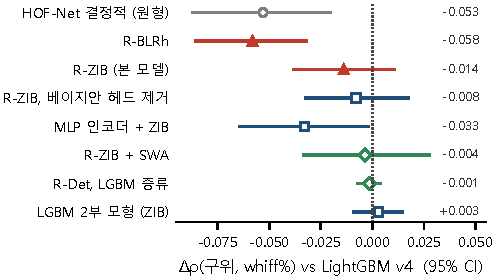
\includegraphics[width=\columnwidth]{figs/fig_forest.pdf}
\caption{LightGBM v4 대비 $\rho_{\mathrm{whiff}}$ 차이와 투수 군집 부트스트랩 95\% 신뢰구간 (시드 42). 대조·진단 실험은 \ref{sec:ablation}–\ref{sec:diag}절.}
\label{fig:forest}
\end{figure}

\subsection{분포 개선의 출처 : 대조 실험}
\label{sec:ablation}
R-ZIB의 분포 예측 개선이 어텐션 인코더와 베이지안 헤드에서 왔는지, ZIB 우도에서 왔는지를 대조 실험으로 분리했다(시드 42). LightGBM의 평균 예측에 같은 방식의 ZIB 헤드를 붙이면 CRPS 0.0732, 0 지점 Brier 0.236으로 R-ZIB(0.0732, 0.235)와 같았다. 0의 확률과 양수 부분을 따로 학습하는 LightGBM 2부 모형도 CRPS 0.0733, $\rho_{\mathrm{whiff}}=0.720$이었다. 즉 분포 예측의 개선은 \emph{우도}의 효과이며, HOF-Net-R 구조 고유의 이득은 아니다. 한편 R-ZIB에서 베이지안 잔차 헤드를 뺀 모형은 $\rho_{\mathrm{whiff}}=0.709$(LightGBM 대비 $-0.008$ $[-0.032,\,0.017]$)로 오히려 약간 높았고, 같은 ZIB 헤드를 다층 퍼셉트론 인코더 위에 둔 모형은 0.684로 신뢰구간이 0 아래였다.

\subsection{순위 격차의 진단}
\label{sec:diag}
R-ZIB와 LightGBM의 순위 격차가 표현력 부족인지 추정 분산인지 진단했다(시드 42). 학습 표본을 10/25/50/100\%로 바꾸면 R-Det의 $\rho_{\mathrm{whiff}}$는 0.595/0.647/0.664/0.681, LightGBM은 0.641/0.680/0.704/0.717로 격차가 0.03–0.05로 유지되었다. 확률적 가중치 평균(SWA)~\cite{izmailov2018averaging}은 R-ZIB를 0.714로, 매개변수를 세 배로 늘린 인코더는 0.712로 올렸다. 가장 결정적인 실험은 증류~\cite{hinton2015distilling}이다. 2025 시즌 505,302구에 대한 LightGBM 예측을 목표로 R-Det을 학습하면 LightGBM 함수를 결정계수 0.96으로 재현하며 $\rho_{\mathrm{whiff}}=0.716$($-0.001$ $[-0.007,\,0.004]$)에 이른다. 같은 인코더가 LightGBM 수준의 함수를 표현할 수 있으므로, 격차의 주원인은 잡음이 큰 목표에서의 추정 분산이다.\footnote{같은 시드 42의 R-ZIB도 GPU(0.704)와 CPU(0.701) 실행이 0.004 다르다. 시드 간 차이보다 작지만, 단일 실행의 0.01 미만 차이는 해석에 주의해야 한다.}

\subsection{불확실성}
공유 가중치의 불확실성 $U_\omega$는 학습 표본을 10\%에서 100\%로 늘릴 때 $1.3\times10^{-5}$에서 $2.5\times10^{-6}$으로 단조 감소했지만, 우연 분산 $U_{\mathrm{ale}}=0.028$의 0.05\%–0.009\%에 불과했다. 구속 98 mph 초과 투구를 95 mph 이하 투구와 구별하는 분포 밖 탐지 AUROC는 R-BLRh의 $U_\omega$ 0.580, $U_{\mathrm{ale}}$ 0.414, R-ZIB의 $U_\omega$ 0.488로 우연 수준이었다. 변분 근사(R-VI)의 사후 표준편차는 닫힌형(R-BLR)의 1.5–2.1배였다. 결론적으로 본 문제에서 Stage II의 베이지안 잔차는 의미 있는 인식론적 불확실성을 제공하지 못하며, 정칙화 이상의 역할을 확인하지 못했다.

\subsection{설명}
그림~\ref{fig:explain}(a)는 2026 시즌 2만 구에 대한 요인 그룹별 기여의 비중이다. HOF-Net-R(5 시드 앙상블)은 LightGBM(TreeSHAP~\cite{lundberg2020local})보다 구속의 비중이 작고(18.0\% 대 28.1\%) 진입각·수평 무브먼트·릴리스 위치의 비중이 크다. 가법성 오차는 $3.3\times10^{-9}$(예측 단위)이었다. 투구별 그룹 기여의 두 모형 간 상관은 0.65(릴리스 위치)–0.95(투구손)였고, 가장 큰 양의 요인이 일치한 비율은 53\%였다. 구종별 단조성 점검에서 포심의 익스텐션은 LightGBM에서 양($+0.57$), HOF-Net-R에서 음($-0.52$)의 기여 방향을 보여 두 모형의 해석이 갈렸다.

배경 수 $K$에 대한 안정성은 그림~\ref{fig:explain}(b)이다. $K=64$ 기준으로 운영 설정 $K=8$의 그룹 기여 상관은 평균 0.953(최소 0.895)이었다. 시드 간 상관은 평균 0.89–0.93으로 LightGBM 재학습 간(0.970)보다 낮아, 설명에도 시드 분산이 남는다. 계산 비용은 CPU 4스레드 1만 구 기준 정확 계산 999초(GPU 약 100초), 순열 근사 111초, LightGBM TreeSHAP 4.5초였고, 순열 근사와 정확값의 그룹 상관은 0.988이었다.

\begin{figure*}[!t]
\centering
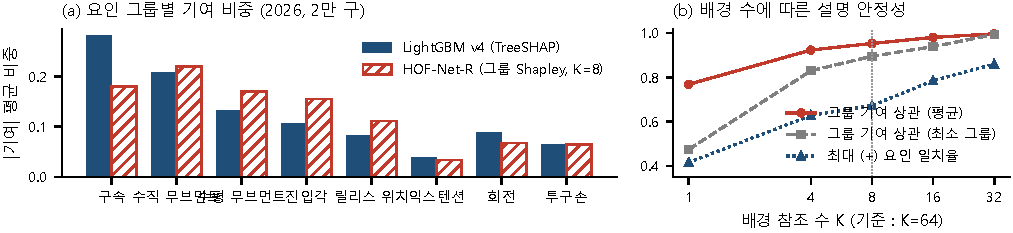
\includegraphics[width=\textwidth]{figs/fig_explain.pdf}
\caption{(a) 2026 시즌 2만 구에서 요인 그룹별 기여 절댓값 평균의 비중. (b) 배경 참조 수 $K$에 따른 HOF-Net-R 설명의 안정성 ($K=64$ 대비). 점선은 운영 설정 $K=8$.}
\label{fig:explain}
\end{figure*}

% ---------------------------------------------------------------------------
\section{운영 적용}
\label{sec:deploy}

HOF-Net-R(R-ZIB)은 2026년 11월 21일부터 구위 분석 웹 서비스의 기본 모형이다. 위 결과는 LightGBM을 대체할 성능 근거를 주지 못하며, 기본 모형 전환은 성능이 아니라 서비스 운영상의 선택이었음을 밝혀 둔다. 11월 27일에는 브라우저에서 같은 점수를 재현하기 위해 5 시드 앙상블을 시드 42 단일 모형으로 바꾸었다. 이때 2025 검증 구간 $\rho_{\mathrm{whiff}}$는 0.7002에서 0.6985로($-0.0017$ $[-0.019,\,0.017]$), RMSE는 0.16818에서 0.16826으로 바뀌었다.\footnote{운영 모형은 $\omega=m$의 결정적 예측이므로, 같은 시드의 연구 비교 값($\omega$ 표본 평균, 0.7006)과 조금 다르다.} 2026 시즌 투수×구종 평균 구위의 앙상블 대비 상관은 0.979, 상위 50쌍 중 39쌍이 유지되었다.

\textbf{브라우저 추론.} 운영 모형의 가중치 81,316개를 float32 그대로 내보내고(압축 0.35 MB), 식~\eqref{eq:block}–\eqref{eq:pred}의 순전파와 식~\eqref{eq:scale}의 척도 변환(4,001점 분위 표의 선형 보간)을 의존성 없는 TypeScript로 구현했다. GELU의 오차함수는 fdlibm 알고리즘으로 배정밀도 구현했다. PyTorch CPU 결과와 비교하면 1,000구(좌투·결측·합성 극단값 포함)에서 $\E[Y]$의 최대 오차 $8.8\times10^{-8}$, 구위 0.0036점, 2026 시즌 실제 투구 20구에서 0.0009점이었다. 한 구의 예측은 0.45 ms, 변수 하나를 41점 격자로 바꾼 반응 곡선은 17 ms에 계산된다(Node.js).

\textbf{가상 투구 해석의 주의.} 반응 곡선은 다른 입력을 고정한 채 변수 하나만 바꾼다. 모형은 입력 간 물리적 상관을 강제하지 않으므로, 예를 들어 좌투 포심의 릴리스 높이만 4.5 ft에서 7.0 ft로 올리면 진입각이 그대로인 채 구위가 47.8에서 상한 80까지 오른다. 학습 분포 밖의 조합에 대한 응답은 근거가 없으므로, 서비스는 입력 범위를 같은 구종의 1–99 분위로 제한하고 이 점을 명시한다.

% ---------------------------------------------------------------------------
\section{논의와 한계}
\label{sec:discussion}

\textbf{기여의 범위.} HOF-Net-R은 원형의 붕괴를 해결하여 LightGBM과 같은 수준의 점 예측에 도달했다. 그러나 대조 실험이 보여 주듯 분포 예측의 개선은 영과잉 Beta 우도의 효과이고, 순위 지표는 약간 낮으며 시드 분산이 크다. 베이지안 잔차 헤드는 측정 가능한 불확실성이나 성능 이득을 주지 못했다. 따라서 본 연구의 실질적 기여는 (i) 약한 신호에서 관측치별 잠재변수가 붕괴하는 기제의 정량적 설명과, (ii) 영과잉 목표에 맞는 우도가 모형 구조보다 분포 예측에 더 중요하다는 실증이다.

\textbf{의사 목표값.} 목표값 $y$는 타구 결과 분류기와 분포 변환으로 만든 의사 목표이므로, 그 편향이 구위에 그대로 전이될 수 있다. 본 연구는 헛스윙률·xwOBAcon·다음 시즌 예측력 같은 외부 지표로 타당성을 확인했지만, 목표값 자체의 불확실성은 모형에 반영하지 않았다.

\textbf{일반화.} 학습은 2025 한 시즌이며, 검증은 시즌 마지막 한 달이다. 신경망은 시드와 실행 하드웨어에 따라 0.004–0.03의 순위 상관 차이를 보였다. 그룹 순위 손실(가중치 0.05에서 $\rho_{\mathrm{whiff}}=0.720$, $+0.003$ $[-0.016,\,0.025]$)과 LightGBM 증류 정칙화가 시드 분산을 줄이는 후보이지만 아직 단일 시드 결과이다. 여러 시즌 학습, 2부 모형, 너무 넓은 예측 구간의 사후 보정이 후속 과제이다.

% ---------------------------------------------------------------------------
\section{결론}
\label{sec:conclusion}
투구 물리량으로 구위를 평가하는 약한 신호·영과잉 회귀 문제에서, 관측치마다 입력 조건부 잠재가중치를 두는 원형 HOF-Net은 KL 비용이 신호의 이득을 넘어 상수 예측으로 붕괴했다. 평균 학습, 전역 베이지안 잔차, 영과잉 Beta 우도로 나눈 HOF-Net-R은 LightGBM과 같은 점 예측과 약 16\% 낮은 CRPS를 얻었지만, CRPS 개선은 우도의 효과였고 순위 지표와 시드 안정성에서는 LightGBM에 미치지 못했다. 정형 데이터의 신경망 확률 모형을 설계할 때, 잠재변수의 정보 예산과 목표값의 지지집합에 맞는 우도를 구조보다 먼저 점검해야 함을 보였다.

% ---------------------------------------------------------------------------
\bibliographystyle{IEEEtran}
\bibliography{refs}

% ---------------------------------------------------------------------------
\appendices
\section{기호}
\label{app:notation}
\begin{center}
\footnotesize
\begin{tabular}{@{}>{\raggedright\arraybackslash}p{0.22\columnwidth}>{\raggedright\arraybackslash}p{0.72\columnwidth}@{}}
\toprule
기호 & 의미 \\
\midrule
$y\in[0,1)$ & 타구질 목표값 (클수록 타자에게 유리, 헛스윙 0) \\
$x$, $p=14$ & 입력 변수와 그 수 \\
$\tilde x_k$, $m_k$ & 표준화 입력, 결측 표시 \\
$Z$, $d=32$ & 토큰 행렬과 토큰 차원 \\
$h(x)\in\mathbb{R}^{448}$ & 평탄화한 인코더 표현 \\
$z(x)\in\mathbb{R}^{r}$, $r=16$ & 잔차 기저, $\tilde z=[z,1]$ \\
$f(x)$ & Stage I 평균 \\
$\omega$, $q(\omega)$ & 공유 잔차 가중치와 그 변분 분포 $\N(m,\mathrm{diag}\,s^2)$ \\
$\tau_0$ & $\omega$의 사전 척도 \\
$\gamma$ & KL 가중치 (1이면 ELBO) \\
$\pi,\mu_+,\kappa$ & ZIB의 0 확률, 양수 부분 평균, 정밀도 \\
$a,b$ & Beta 형상 모수 $a=\mu_+\kappa$, $b=(1-\mu_+)\kappa$ \\
$\sig$ & 로지스틱 함수 \\
$U_{\mathrm{ale}},U_\omega$ & 우연 분산, 공유 가중치의 분산 \\
$s(x)$ & 20–80 구위 점수 \\
$W_i$, $q_\phi,p_\psi$ & (원형) 투구별 잠재가중치, 변분·사전분포 \\
$\rho_{\mathrm{whiff}}$ & 투수×구종 평균 구위와 헛스윙률의 순위 상관 \\
\bottomrule
\end{tabular}
\end{center}

\section{초매개변수}
\label{app:hparam}
\begin{center}
\footnotesize
\begin{tabular}{@{}>{\raggedright\arraybackslash}p{0.30\columnwidth}>{\raggedright\arraybackslash}p{0.64\columnwidth}@{}}
\toprule
항목 & 값 \\
\midrule
인코더 & 토큰 $d=32$, pre-LN 블록 2개, 4헤드, FF $32\to64\to32$, GELU, 드롭아웃 0.1 (어텐션 가중치 제외) \\
잔차 기저 & $448\to64\to16$, GELU, 드롭아웃 0.1 \\
Stage I & 표준화 목표 MSE, AdamW (lr $10^{-3}$, wd $10^{-4}$), 배치 1,024, 최대 30 epoch, 인내 4, 기울기 노름 5 \\
Stage II & $\tau_0\in\{0.01,\dots,3\}$ 중 홀드아웃 NLL 최소 (모든 시드 0.01); 분산 헤드 $16\to32\to1$; 변분 학습 Adam lr $10^{-2}$, 배치 4,096, 15 epoch \\
Stage III & ZIB 헤드 $448\to64\to64\to3$, $\kappa_{\min}=10^{-3}$, $\tau_0=1$, 배치 1,024, 최대 30 epoch, 홀드아웃 ZIB NLL 조기 종료 \\
설명 & 8개 그룹, 층화 배경 $K=8$, 정확 256 부분집합 / 순열 4개 \\
시드 & 42–46 (운영 모형 42) \\
\bottomrule
\end{tabular}
\end{center}

\end{document}
